\documentclass{beamer}

\usepackage[utf8]{inputenc}
\usepackage{graphicx}
\usepackage{mathtools}
\graphicspath{ {img/} }
\usetheme{Berlin}
\usecolortheme{Crane}

\title[Learning Linux]{Linux: The Command Line}
\author{Jacob Beal}
\date{\today}
\begin{document}
\frame{\titlepage}
\begin{frame}
    \frametitle{Why use the command-line?}
    \begin{itemize}
        \item<1-> More Powerful
        \item<2-> Faster
        \item<3-> Not all programs have graphical interfaces
        \item<4-> Street-Cred
    \end{itemize}
\end{frame}
\begin{frame}
    \frametitle{Quick tip for people on Laptops}
    \begin{block}{Windows}
    Download PuTTY \url{http://www.chiark.greenend.org.uk/~sgtatham/putty/download.html}
    \end{block}
    \pause{}
    \begin{block}{OS X}
    Open a terminal and use ssh.
    \end{block}
\end{frame}
\begin{frame}[fragile]
    \frametitle{SSH into Lab computers: OS X}
    The following into a terminal session:\\
    \verb|ssh |$\underbrace{bealjaco}_\text{Your ECS username}$\verb|@greta-pt.ecs.vuw.ac.nz|
\end{frame}
\begin{frame}[fragile]
    \frametitle{SSH into Lab computers: Windows}
    Open up the \verb|putty.exe| that you downloaded earlier
    \begin{center}
        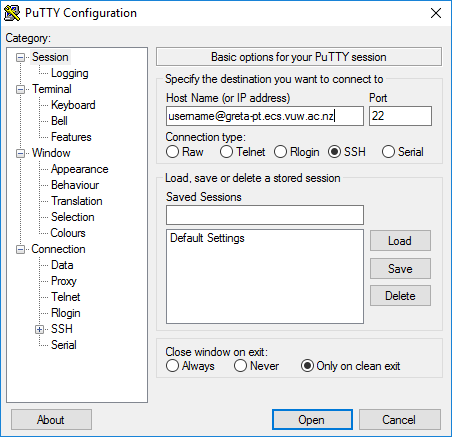
\includegraphics[width=0.4\textwidth]{putty}
    \end{center}
    Then type in your password etc\ldots to get into the shell of the
    University computers
\end{frame}
\begin{frame}[fragile]
    \frametitle{Quick Set-Up}
    Type the following in the command line just to set-up the example files, so
    we are all working with the same files:\\
    \verb|git clone git@github.com:jb567/linux-guide.git|\\ %TODO: Confirm the git repo
\end{frame}
\begin{frame}[fragile]
    \frametitle{Navigation: Changing Directory}
    The command to change directory is \verb|cd|.\\
    The syntax of this command is `\verb|cd folder|'
    \begin{example}
        \verb|cd| $\underbrace{\textit{terminal-tut-files}}_\text{folder you
            want to navigate to}$\\
        \verb|cd| is a shortcut for \verb|cd ~|
    \end{example}
    \pause{}
    \begin{alertblock}{Misnavigation with /}
        if you use a folder and put a \verb|/| before the foldername it goes to
        the \textit{root} of your file system.
    \end{alertblock}
\end{frame}
\begin{frame}[fragile]
    \frametitle{Navigation: Where am I?}
    There are a few ways of knowing where you are:
    \begin{itemize}
        \item<1-> \verb|greta-pt: [~] | is on the left hand side of your
            terminal. The address within the square brackets is where you are,
            normally relative to the \verb|~| directory            
        \item<2->Use the command \verb|pwd|. This will just output where you are
            relative to the `root directory'
        \begin{alertblock}{What is the \textasciitilde{} and root  directory}<3->
            The \textasciitilde{} directory is your `home' directory.\\
            This is typically your user folder.\\
            The `root' directory is the base folder in your file system.\\
            Think of it like the \verb|C:\| directory on Windows.
        \end{alertblock}
    \end{itemize}
\end{frame}
\begin{frame}[fragile]
    \frametitle{File Manipulation: Move a File}
    So you can move around the file tree, now what about files?\\
    \begin{block}{mv command}<1->
        The \verb|mv| command takes the arguments as follows:\\
        $$\text{mv}\ \underbrace{\textit{source\_file}}_\text{File you want to move}\ \underbrace{\textit{target\_location}}_\text{Where you want to move it to}$$\\
    \end{block}
    \begin{example}{Example}<2->
        
    \end{example}
\end{frame}

\end{document}
